\documentclass{mcmthesis}
%\usepackage[justification=center]{caption}%表格标题居中
\usepackage{booktabs}%粗表格

\usepackage{indentfirst}%首行缩进
\usepackage{graphicx}%图片
\usepackage{subfigure}
\usepackage{url}

\mcmsetup{tcn = 85691,problem = B,titlepage = false}
\title{Use Diffusion Models to Solve the Problem of Language Communication}
\begin{document}

\setlength{2em}%设置段首行缩进2字符{parindent}

  \begin{abstract}

    \ \ A multinational service company needs a report about trends in global languages and an office site-selection plan.
    We need to sort out the factors that influence the transmission of the language and predict the trends of language transmission.
    Finally, we should provide a site-selection plan.

    Fick's Law is used in material science to describe substance diffusion.
    And we refer to the law establish a language diffusion model.
    Just like the diffusion process that ink is added to water.
    We use coloured circle refer to people who can speak a particular language, and other places on the plane refer to those who can not speak the language.
    The process of colour diffusion in the plane is just like the process of language transmission. So in this way,
    we can calculate the number of speaker.
    We also analyze the impact of population, GDP and immigration on the transmission of language.
    Then we study geographic distribution of language using some particular countries.
    In order to find the suitable places for offices,
    we establish a value function and use an iterative method to find a local optimal solution.

    According to our model, the change of population,
    similarities between different languages,
    immigration and economic conditions all play important role in language transmission.
    And we find that the number of English speaker grow faster than any other language in the next fifty years.
    Arabic and Hindustani will also develop rapidly in future,
    while other languages will not have much change.
    In different continents, the geographic distributions of language are not the same.
    We suggest that the multinational service company could set up offices in the UK, India, the Arab World, France, Mexico and Brazil.
    If only five offices are available, we could remove Mexico from the list.

    We evaluate the sensitivity of the model.
    When we change the value of GDP, the predicted results have significant changes.
    So it shows that the economy could help the transmission of language.
    When we predicting the value,
    the bigger number of iterations,
    the bigger the prediction.
    So we could get a better result if we use multiple fitting.

    Our model has great adaptability.
    When we change some situations,
    such as GDP, immigration and population,
    the predicted value could change,
    which reflects the objective law.

    The weakness of our model is that we have to predict GDP and the number of immigration first.
    And then using them to predict language transmission.
    So it could increase the model's error.

  \end{abstract}

  \maketitle
  \tableofcontents

  \clearpage%另起一页
  \section{Introduction}%引言
    \subsection{Background}
    With the development of society, we now have more and more opportunities to communicate with people from different cultural backgrounds.
    It is undoubtedly a good thing for us whether for our personal ability to enhance or the country's economic and cultural communication.
    But there are some issues we have to overcome.
    And language is one of the issues.
    When we can't communicate with other people using a language we are familiar with,
    I'm sure that it will be a tough situation.
    Because of so many advantages the cross-cultural economic and cultural exchanges could bring to us,
    I think we should pay more attention to how to choose a language to communicate.

    It is always not an easy job to select a suitable language for people to communicate.
    When a language is selected, we may spend time and money learning a new language.
    And for businesses, a suitable language means efficient communication, which means maximizing profits.
    From our view, in order to make a choice,
    we should search the information about the current usage of various languages
    and what's more important is predicting the future development of different languages.

    However, predicting the future,
    especially when we need a long-term forecast and are in the absence of data,
    is very difficult.
    Therefore, we want to use the model from other study fields to solve our problem.
    And we find that there are some similarities between the spread of language and substance diffusion.
    So we try to use the substance diffusion model to illustrate the puzzle about linguistics.

    \subsection{Assumptions}%假定

    \begin{enumerate}

    \item Only a few countries could include the vast majority of language users
    \item Immigrants can use the main language in the destination
    \item Immigration does not have much impact on the national population
    \item The main language is a language is used by the most people in a country
    \item There is no more than one office in a country
    \end{enumerate}


    \subsection{Terminology}%术语

    \begin{table}[h]
      \centering
      \caption{Notation}

      \begin{tabular}{cc}
        \toprule%line
        Symbol&Meaning\\
        \midrule%line
        {$D$}&Diffusion Coefficient\\
        {$Total$}&Total Numbers of Speakers\\
        {$Total'$}&Total Numbers of Speakers After a While\\
        {$L_1$}&Number of the Native Speakers\\
        {$L_1'$}&Number of the Native Speakers After a While\\
        {$L_2$}&Number of the Second Language Speakers\\
        {$L_2'$}&Number of the Second Language Speakers After a While\\
        {$k_0$}&Integration Upper Bound\\
        {$Imm$}&Immigration\\
        {$LF$}&Language Family\\
        {$W$}&Office Location Program Value\\
        {$w_i$}&the i-th Office's Regional Value\\

        \bottomrule%line
      \end{tabular}
    \end{table}



  \section{The Models}
  We study the first language and the second language change.
  A person's native language will not change.
  \begin{enumerate}
  \item The Language Diffusion Model is an all-encompassing foundation that describes the overall change in language usage across the world.
  At the same time, it is used to solve the second question.

  \item The Analysis of Influencing Factors is to find the influencing factors in the process of language diffusion.
  The number of first languages is affected by demographic changes.
  We look at the change in the number of second languages from another perspective.
  The consequence of language communication is that people learn a new language.
  That is the second language change.
  At the same time, the influencing factors model is used to solve the first question.

  \item Language Distribution in some Specific Areas describes the distribution of changes in various languages in a particular country or region.
  It is used to solve the third question.
  At the same time, it is also a factor for site selection.

  \item Model of Setting Up Office is used to quantify the benefits of the office selection.
  It is used to solve the fourth question and fifth question.
  \end{enumerate}

    \subsection{Language Diffusion Model}%语言扩散模型
    \subsubsection{Traditional Diffusion: Fick's Second Law}%传统扩散:菲克第二定律

    Fick's law is a quantitative formula developed by Fick in 1858
    with reference to the Fourier heat conduction equation
    to describe the migration of substances
    from a high concentration region to a low concentration region.
    Fick's second law describes the state as follows
    when the concentration of diffusate varies with time at any point in the diffusion medium,
    that is, the distribution of concentration gradients throughout the system is dynamic:
    $$\frac{\partial C}{\partial t}=D\frac{\partial^2C}{\partial x^2}$$

    Where $C$ is the concentration, $x$ is the coordinate, and $t$ is the time.

    It gives a mathematical expression of the diffusion of matter in the medium.
    We use it to calculate the concentration of each point,
    and integral it to calculate the amount of material.

    $D$ is called the diffusion coefficient.
    It is related to the physical properties of diffusion media and dispersions.
    And it is also a decisive factor in determining the speed of proliferation.
    The larger the $D$, the greater the rate of diffusion.
    \subsubsection{Transform It into the Language Diffusion Model}%将扩散模型转化到语言扩散模型

    Firstly we use a plane to refer to the entire human possession of space.
    We think the area of this plane is limited, and the area is equal to the total human population.
    Of course, this area is also changing
    Then the person who uses the A language is a circle in the center of the plane.
    The area of this circle is the total number of people who use the A language (including the first language and the second language).
    Refer to Figure 1.
    %\ref{p1}

    The expansion of the total number of languages is the process of increasing color.
    In the model, it is the color slowly from the color circle into the plane of the blank, like ink dripping into water slowly spread the same.
    Please note here that the boundary of the circle after diffusion becomes unclear.
    In order to achieve the model's computability, we define a parameter $k$.
    For example: $k=60\%$.
    Take a ring with a color concentration of 60% as a circle border.
    Integrate this ring from the original color circle boundary to the new one.
    We get the number of people who have proliferated.
    This number is an increase in the number of second language
    (Changes in the number of speakers in the first language are related to changes in the population that mainly use the language.)
    This diffusion process is governed by two factors: the circumference of the initial color circle and the rate of diffusion.

    \begin{figure}[h]
      \begin{minipage}[t]{0.5\linewidth}
      \centering
      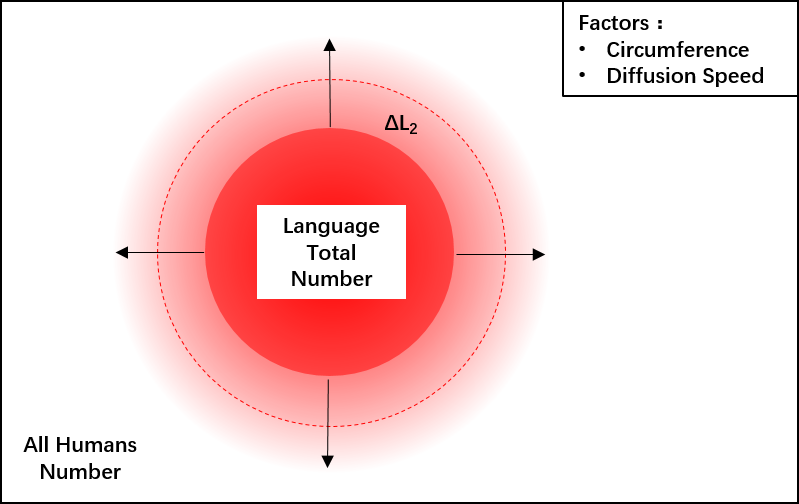
\includegraphics[height=3.8cm,width=6cm]{p1.png}%height=2.4cm,width=3.8cm
      \caption{Language Diffusion Model}
      \label{p1}
      \end{minipage}
      \begin{minipage}[t]{0.5\linewidth}
      \centering
      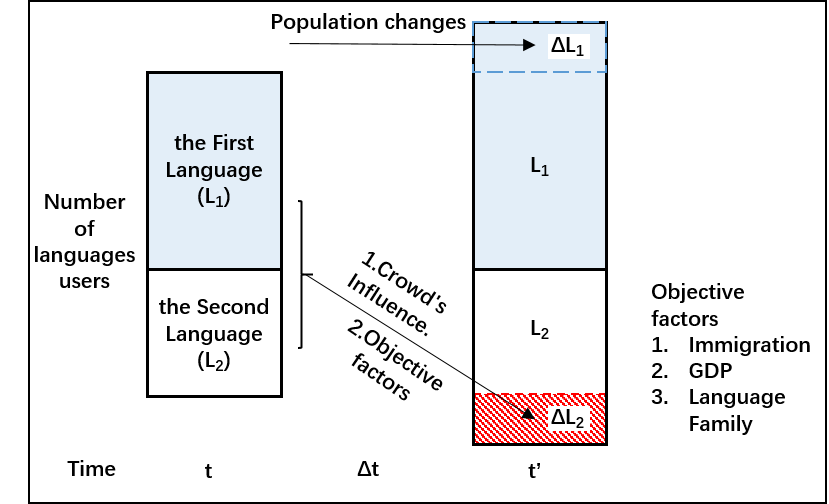
\includegraphics[height=3.8cm,width=6.3cm]{p2.png}%width = .48\linewidth
      \caption{Changing Way in Speakers}
      \label{p2}
      \end{minipage}
    \end{figure}

    %\begin{figure}
      %\centering
      %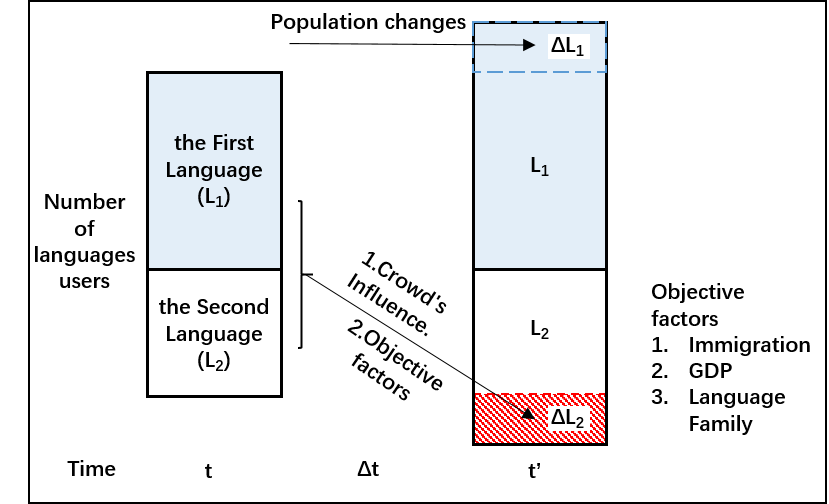
\includegraphics{p2.png}
      %\caption{Changing Way in Speakers}
      %\label{p2}
    %\end{figure}

    The total number of language changes is divided into two parts, one is the number of changes in the first language, another is the number of changes in the second language.
    Whether it is studying immigrants, work or government incentives, are only increased the number of second languages.
    Therefore, the number of first languages is only related to the growth of the population of many countries that mainly use this language.
    The growth of a second language is related to the overall influence of the language, including the number of people using the language and the objective factors.
    Then the number of speakers, the larger the corresponding area, the greater the side length.
    This indicator quantifies the crowd's influence.
    Objective factors determine the speed of diffusion.
    We use the diffusion coefficient $D$ to quantify it.
    Furthermore, we analyze the GDP, linguistic systems and the impact of immigrants on the diffusion coefficient in the major countries that use languages.
    This represents the degree to which people in real life learn the language.
    Refer to Figure 2.

    As the number of languages used is too large (hundred million),
    the effect of the number of people who grew over time on the radius of the circle is negligible.
    At this point we can approximate the ring as a rectangle.
    We do not consider differences in proliferation in all directions.
    Then we can calculate the diffusion effect of a line,
    and then multiply the circumference of the original color circle
    to get the number of people added, that is, the " Concentration Area " of the circle.
    "Concentration Area" means that the coloring of this ring is not uniform.
    The actual area is not equivalent to the actual number.
    Take the proportion of people who use the A language per unit area as the concentration $C$.
    Refer to Figure 3.

      \begin{figure}[h]
        \centering
        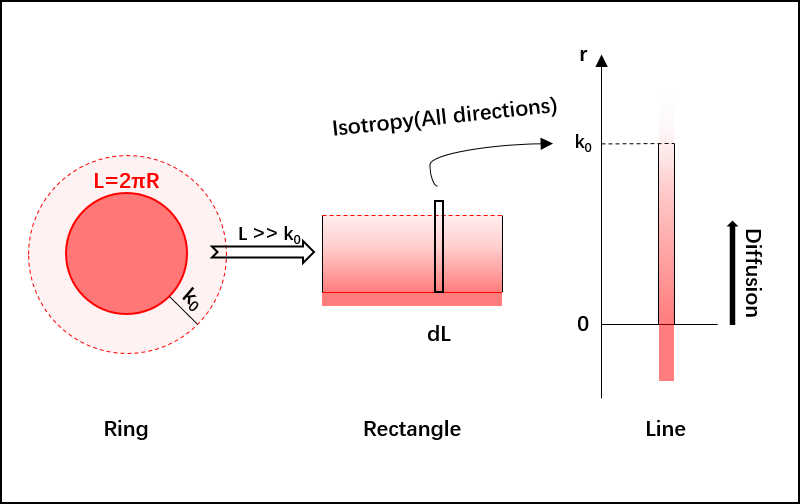
\includegraphics[height=6.3cm,width=10cm]{p3.png}
        \caption{Approximate Replacement Process}
        \label{p3}
      \end{figure}

    Here we solve this situation.
    Fick's second law is a partial differential equation.
    We try to turn it into an ordinary differential equation.
    We suppose that the concentration of the colored circles is constant and then deduced:
    \\Initial conditions: \ \ \ \ \  When \ \ \ $t=0$\ ,\ $x\approx 0$,\ $C_{(x,t)}=0$
    \\Boundary conditions: When \ \ \ \ $t>0$\ ,\ $C_{(0,t)}=1$%\textgreater
    \\Using Boltzmann transformation:
    $$\lambda=\frac{x}{\sqrt{t}}$$
    Substitute Fick's second law:
    $$-\lambda\frac{{\rm d}C}{{\rm d}\lambda}=2D\frac{{\rm d}^2C}{{\rm d}\lambda^2}$$
    After substitution, suppose $\beta=\frac{\lambda}{2\sqrt{D}}=\frac{x}{2\sqrt{Dt}}$ ,
    the result of the final integration is:
    $$C_{(x,t)}=a\int_0^\beta exp(-\beta)^2{\rm d}\beta+b$$
    The integral $\int_0^\beta exp(-\beta)^2{\rm d}\beta$ is called Gaussian error function.
    According to Gaussian error function:
    $$\int_0^\infty exp(-\beta)^2{\rm d}\beta=\frac{\sqrt{\pi}}{2}$$
    Consider initial conditions and boundary conditions:
    \\When $x\rightarrow\infty$,\ then $\beta\rightarrow 0$,\ $C_{(\infty,t)}=a\frac{\sqrt{\pi}}{2}+b=0$
    \\$x=0$,\ then $\beta=0$,\ $C_{(0,t)}=b=1$,then:
    $$a=-\frac{2}{\sqrt{\pi}},b=1$$

    The final concentration equation is:
    $$C_{(x,t)}=1-\frac{2}{\sqrt{\pi}}\int_0^\beta exp(-\beta)^2{\rm d}\beta=1-erf(\frac{x}{2\sqrt{Dt}})$$

    In our model,\ $r$ represents the distance to the colored circle border.
    So we replace $r$ with $x$ :
    $$C_{(r,t)}=1-erf(\frac{r}{2\sqrt{Dt}})$$
    We integrate this concentration function.
    As mentioned earlier, in order for the results to be presented, we agree on a ratio $k$.
    The ring of concentration $k$ is the upper bound of the integral.
    $k$ corresponding to the distance $k_0$ obtained by the formula:$C_{(k_0,t)}=k$
    \\Then the final increment of the second language ($\Delta L_2$) is expressed as:
    Concentration Integral × Colored Circle Circumference
    $$\Delta L_2=\int_0^{k_0} C_{(r,t)}{\rm d}r\times 2\pi\sqrt{\frac{Total}{\pi}}=\int_0^{k_0}(1-erf(\frac{r}{2\sqrt{Dt}})){\rm d}r\times 2\pi\sqrt{\frac{Total}{\pi}}$$

    Furthermore, given a predictive time $t$ after determining $D$ based on objective factors,
    we can make a numerical prediction of the growth of future second language populations.
    Combined with the population growth trend of the first language of the number of predictions,
    we can predict the future of a language of the total number of years.
    $$Total'=L_1'+L_2+\Delta L_2$$



    \subsection{Analysis of Influential Factors}%语言传播的影响因素
    A large number of objective factors will affect the spread of language.
    From the foregoing description, we can see that the value of the diffusion coefficient $D$ determines the number of second language population changes.
    After reviewing the relevant literature and some life experiences, we have made some discoveries
    We can set the language-specific diffusion coefficient $D$ to be relevant to the economy of the country
    where the language is dominant and also to the number of immigrants who master the language.
    At the same time, the ease of learning this language can affect the number of the second speakers.
    We call it the impact of language on Language Family.
      \subsubsection{GDP}
    For the convenience of calculation and discussion, we select for each language a specific country or countries to represent all countries in which that language is the primary language.
    Here we select a total of 20 countries and organizations.
    For the economy behind the language, we use the sum of some specific countries GDP figures.
    For the convenience of calculation in the next step, we will use the GDP ratio.
    The formula is as follows:
    $$GDP=\frac{\sum GDP\ \ \ (Specific\ \  Countries)}{\sum_{20} GDP\ \ \ (All\ \  Countries)}$$


    \subsubsection{Imm:\ Immigration}%移民
    The number of immigrants can also reflect the number of second language speakers on the one hand.
    Here we can emigrate to the United States as an example.
    In order to migrate smoothly, we must master English as a second language.
    The U.S. government and people's attitude toward immigration and
    the U.S. economy are important references in deciding whether or not we immigrate to the United States.
    So we use Equation $h\times GDP$ to show how attractive a particular country is to immigrants.
    Where, $h$ is a categorical variable.
    $$Imm=\frac{\sum h\times GDP\ \ \ (Specific\ \  Countries)}{\sum_{20} h\times GDP\ \ \ (All\ \  Countries)}$$
    \subsubsection{LF:Language Family}%语系
    In terms of language difficulty,
    we use the classification of the U.S. Department of State's
    " Report to Congressional Requesters:
    Foreign Language Proficiency Has Improved, but Efforts to Reduce Gaps Need Evaluation"
    which divides the language into four categories, with assignments of 0.25, 0.5, 0.75 and 1 respectively.

    We studied 7 languages.
    The specific classification is as follows:


    \begin{table}[h]
      \centering
      \caption{Language Classification}

      \begin{tabular}{cccc}
        \toprule%line
        1&0.75&0.5&0.25\\
        \midrule
        Category\uppercase\expandafter{\romannumeral1}&Category\uppercase\expandafter{\romannumeral2}
        &Category\uppercase\expandafter{\romannumeral3}&Category\uppercase\expandafter{\romannumeral4}\\
        World languages&Difficult world languages&Hard languages&Super-hard languages\\
        \midrule%line
        English&&Russian&Arabic\\
        French&&Hindustani&Mandarin Chinese\\
        Spanish&&&\\
        Portuguess&&&\\
        \bottomrule%line
      \end{tabular}
    \end{table}

    We assume that $D$ is only determined by the above three factors.
    $D$ is expressed as the following equation:
    $$D=\beta_1\times Imm+\beta_2\times GDP+\beta_3\times LF$$





    \subsection{Language Distribution in some Specific Areas}%特定区域的语言分布情况
    %轲轲
    In general, first language speakers are only active in certain geographical areas
    generally within the same country.
    And our changes to the geographical distribution of languages are at the national level.
    We assume that the first language speaker has no influence on the geographical distribution of the language.
    Only the second language has an impact on the geographical distribution of the language.

    At the same time the second language is divided into two categories.

    We take the geographical distribution of Chinese as an example.
    We define the first language as a native speaker and the second language as a second language speaker.
    We use $L_{21}$ refer to him.
    We define the native language as English and the second language as Chinese as second language.
    We use $L_{22}$ refer to him.
    The first type of immigrants to English-speaking countries (U.S.) made the number of Chinese speakers in the geographic area of the United States increase.
    At the same time, a second type of people living in the United States, the number of Chinese in the United States geographical area also increased.

    By language diffusion model, we can get the number of the second language of the future specific language.
    For some time, the increase in the number of second languages was the increase in the number of immigrants and those in Category\uppercase\expandafter{\romannumeral2}.
    For immigrants, we can calculate the immigrants and emigrants of 20 countries by referring to the data of UNIDO (United Nations Industrial Development Organization ).
    For the second person, $\Delta L_2=L_2'-L_2$\ \ $\Delta L_2- L_{21}= L_{22}$\\
    $\Delta L_2$ is the added value of Chinese as a whole.
    We can allocate $\Delta L_2$ based on the ratio of the population of each country to the total population of 20 countries.
    After distribution, calculate the number of $L_{22}$ in the United States.Refer to Figure 4.
    The formula is as follows:
    $$L_{22}(U.S.)=\frac{Population(U.S.)}{\sum_{20}Population(All Countries)}\times L_{22}$$
    \begin{figure}[h]
      \centering
      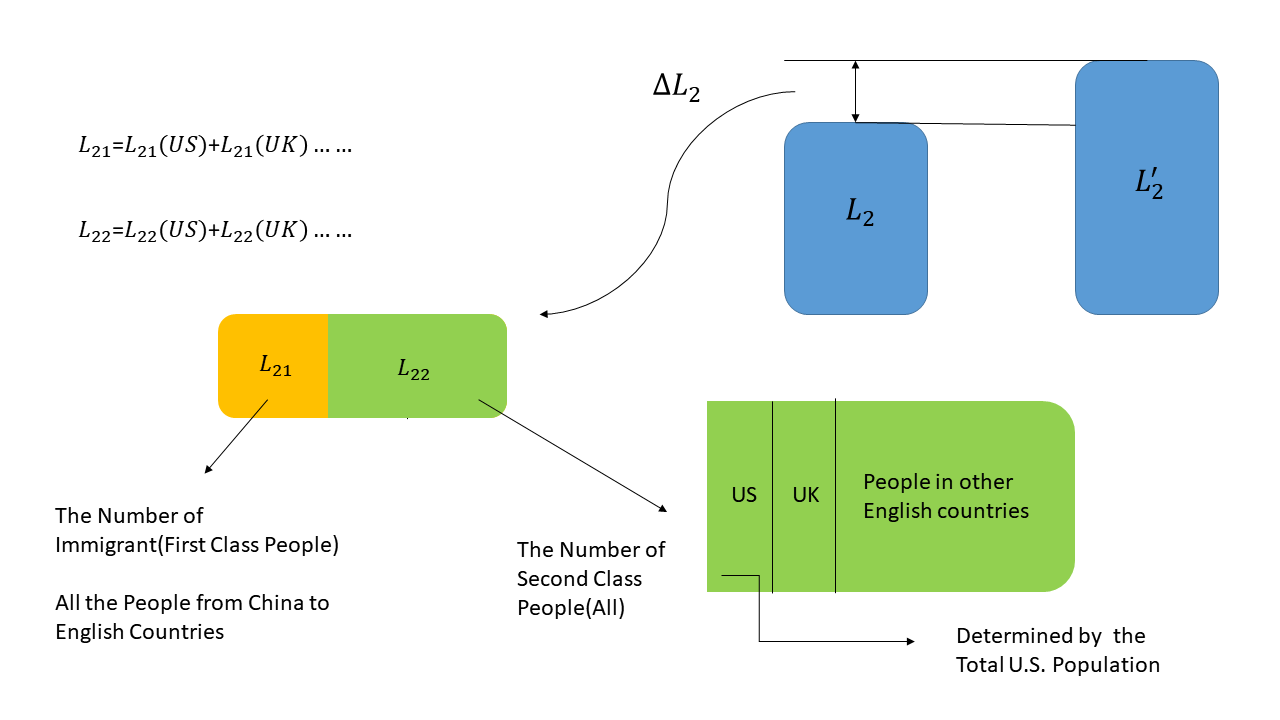
\includegraphics[height=6.3cm,width=10cm]{p7.png}
      \caption{Relationship of $\Delta L_2\ \ L_{21}\ \ L_{22}$\ \ and \ \ $L_{22}(U.S.)$ }
      \label{p7}
    \end{figure}

    Now you can get the number of annual growth in 20 countries in 8 languages.
    Thus infer the change of its geographical distribution.




    \subsection{Model of Setting Up Office}%办事处的设立方法

    The statistical analysis we did above shows how language changes its distribution with time, space and population.
    According to statistical economic and linguistic factors, we selected 20 representative countries and regions as the research object. At this point, we have simplified the issue to choosing six of the 20 countries that we are interested in to set the new offices.
    Generally, there are two main factors we have to consider while selecting the right spots:

    \begin{enumerate}
      \item The location's value to the company.
      \item The influence between two offices.
    \end{enumerate}

    To quantify the value of the 20 countries to the company,
    we set up an evaluation system that addresses the region's GDP, population, and various second language growth.
    We calculate the standardized population, language, and economy for each area.
    We weighted averages the three parameters to get the value score of the region.

    Next we calculate the weight.
    We calculate the Standard Deviatio of the data distribution of the three parameters respectively.
    The Standard Deviatio is used as the weight of each parameter.
    GDP use of GDP ratio.
    Population use of Proportion of the population.
    Language uses a new indicator.
    It is calculated as follows:
    $$L(Language)=\frac{\sum \Delta Total(The Language)\ \  (Specific Area)}{\sum_{20} \Delta Total(The Language)\ \  (All Areas)}$$

    We will be three evaluation indicators by weight as a quantitative indicator.
    The meaning of the result is: the greater the value, the higher the value of the area.

    We have a unique perspective on the interplay between offices.
    It would be a waste to set two offices in the same country when the total amount of office is limited.
    Once two offices are set too close, their services areas may overlap.
    This makes some resources could not be fully utilized, resulting in the waste of resources.
    In conclusion, The distance between two offices should be as far as possible.
    We found the latitudes and longitudes of capitals or important cities
    in these 20 regions to use the distance between cities to represent the distance between regions.

    Assuming there is 6 new offices need to be set, that is to say, the total number of the office is 8.
    Let $d_{ij}$ denote the distance between the i-th office and the j-th office.
    Let $w_i$ be the i-th office's regional value.
    Then the value of this program W is:
    $$W=\sum_{i=1}^8(w_i\frac{\sum_{j=1,j\neq i}^8 d_{ij}}{8})$$

    We will use this function as a value function to quantify the location of the office.

    We can give a feasible solution first.
    Since there are already two offices set in new York and Shanghai,
    the initial feasible solution is the top six countries.
    Use the formula above and we can get a $W$.
    Then we optimize.
    After alternating the ninth region with the six regions added earlier,
    we can calculate six post-exchange $W'$.
    If there are $W'>W$ solutions in the 6 exchanges,
    then the new state is taken as a new feasible solution,
    and if not, the iteration is stopped.



  \section{Models Calculation}%模型计算

    \subsection{Calculate Diffusion Coefficient $D$ Based on Historical Data}%根据历史数据计算扩散系数
    When $k$, $t$, $Total$ given, $\Delta L_2$ is only a function of $D$.
    We can, in turn, find the diffusion coefficient $D$,
    for a given time period in a given language based on $\Delta L_2$.
    The calculation results are as follows:

    \begin{table}[h]
      \centering
      \caption{Diffusion Coefficient}

      \begin{tabular}{cccc}
        \toprule%line
        Language&$D_1$(2015--2017)&$D_2$(2013--2015)&$D_3$(2008--2013)\\
        \midrule%line
        Mandarin Chinese&0.003163&0.1582&--\\
        English&0.02494&12.1727&13.6771\\
        Hindustani (Hindi/Urdu)&1.2009&0.3726&0\\
        Spanish&0.006543&0.7769&--\\
        Arabic&1.6014&--&--\\
        Russian&0&0&--\\
        French&0.2827&14.1057&0\\
        \bottomrule%line
      \end{tabular}
    \end{table}

    \subsection{Prediction of Language Speakers after 50 Years}
    We found that the same statistical method does not have to be used for the data of language speakers in Wiki or Ethnography.
    This phenomenon was remarkable at the beginning of the 20th century.
    We choose seven better language data to predict.

    Assuming that in these 50 years, the objective factors remain largely unchanged.
    We select the most appropriate one of the diffusive coefficients $D$ that have been found.
    Apply this model to calculate the growth of $L_2$ according to this diffusion coefficient.
    $$\Delta L_2=\int_0^{k_0}(1-erf(\frac{r}{2\sqrt{Dt}})){\rm d}r\times 2\pi\sqrt{\frac{Total}{\pi}}$$
    We use population projections to calculate the change in the number of first-language speakers in 50 years,
    iterate through the model $Total'=L_1'+L_2+\Delta L_2$ and finally calculate the total number of speakers of a certain language after 50 years.

    We choose to iterate five times.
    Then we plot the line chart for the iteration in seven languages on the same chart.
    The result is as follows:
    \begin{figure}[h]
      \centering
      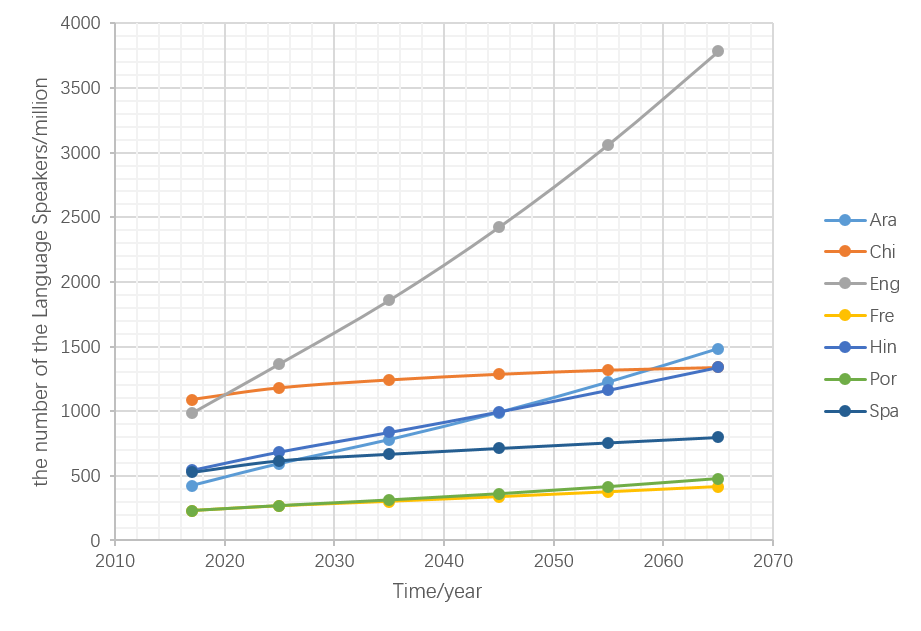
\includegraphics[height=6.3cm,width=10cm]{p4.png}
      \caption{Prediction of Language Speakers after 50 Years}
      \label{p4}
    \end{figure}

    \subsection{Calculation of Language Distribution in some Specific Areas}
    %轲轲
    Based on the model and the calculated standardized immigration, GDP and population data,
    we predict the language distribution of different countries or regions in the future.
    Specifically, we calculated the increase in the number of second language speakers in seven major languages at some point in the future.
    In order to better reflect the results, we use the statistics of the continent as a unit and present it as a line chart.
    The abscissa is the year, and the ordinate is the number of changes.
    The results presented in the Figure 6 to Figure 11.

    \begin{figure}[h]
      \begin{minipage}[t]{0.5\linewidth}
      \centering
      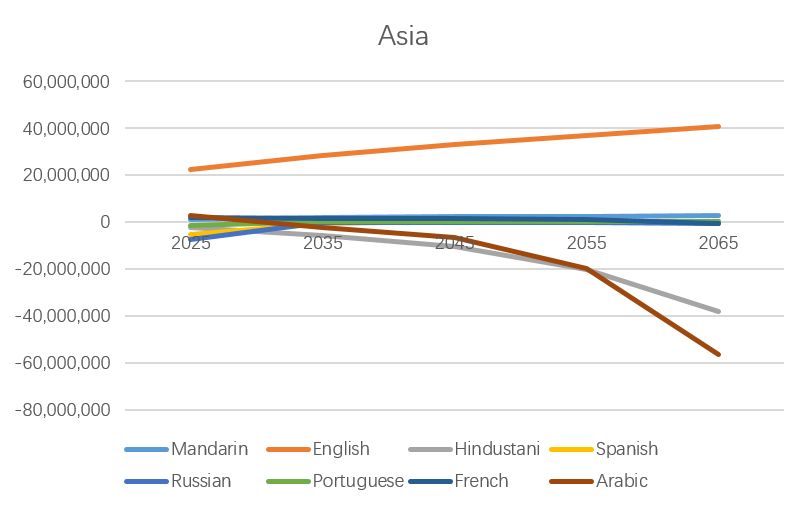
\includegraphics[height=3.8cm,width=6cm]{A01.png}%height=2.4cm,width=3.8cm
      \caption{Asia Language Distribution}
      \label{p8}
      \end{minipage}
      \begin{minipage}[t]{0.5\linewidth}
      \centering
      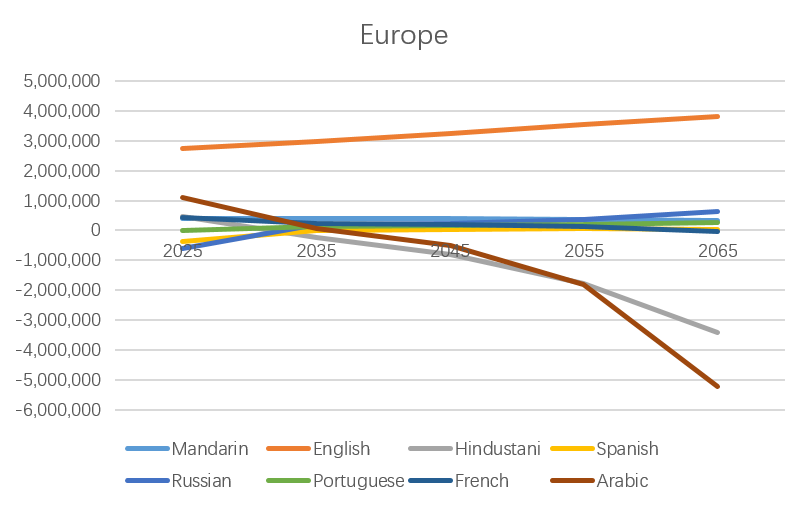
\includegraphics[height=3.8cm,width=6.3cm]{A02.png}%width = .48\linewidth
      \caption{Europe Language Distribution}
      \label{p9}
      \end{minipage}
    \end{figure}

    \begin{figure}[h]
      \begin{minipage}[t]{0.5\linewidth}
      \centering
      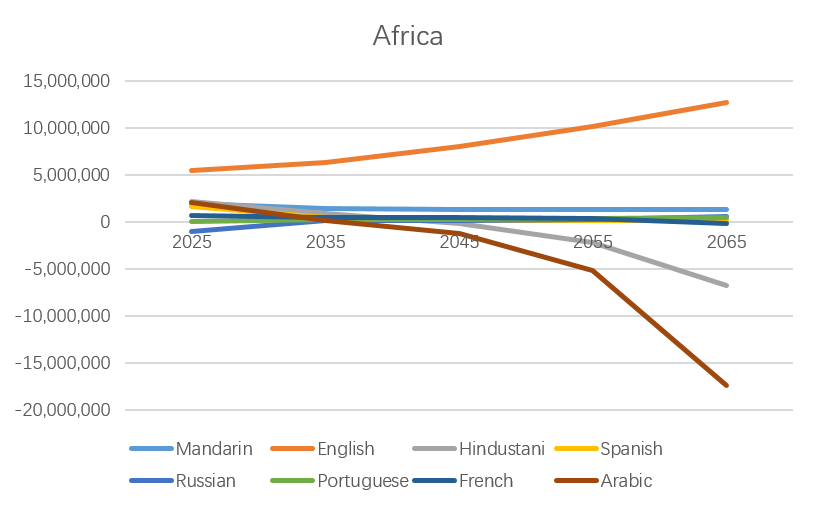
\includegraphics[height=3.8cm,width=6cm]{A03.png}%height=2.4cm,width=3.8cm
      \caption{Africa Language Distribution}
      \label{p10}
      \end{minipage}
      \begin{minipage}[t]{0.5\linewidth}
      \centering
      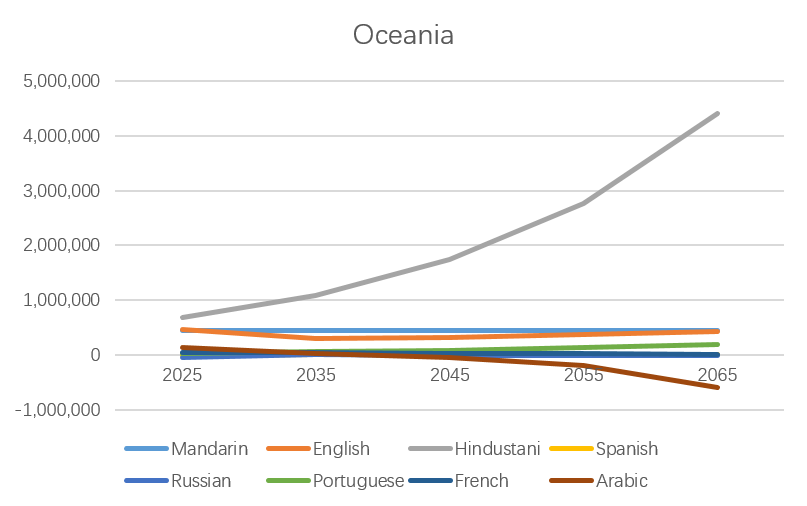
\includegraphics[height=3.8cm,width=6.3cm]{A04.png}%width = .48\linewidth
      \caption{Oceania Language Distribution}
      \label{p11}
      \end{minipage}
    \end{figure}

    \begin{figure}[h]
      \begin{minipage}[t]{0.5\linewidth}
      \centering
      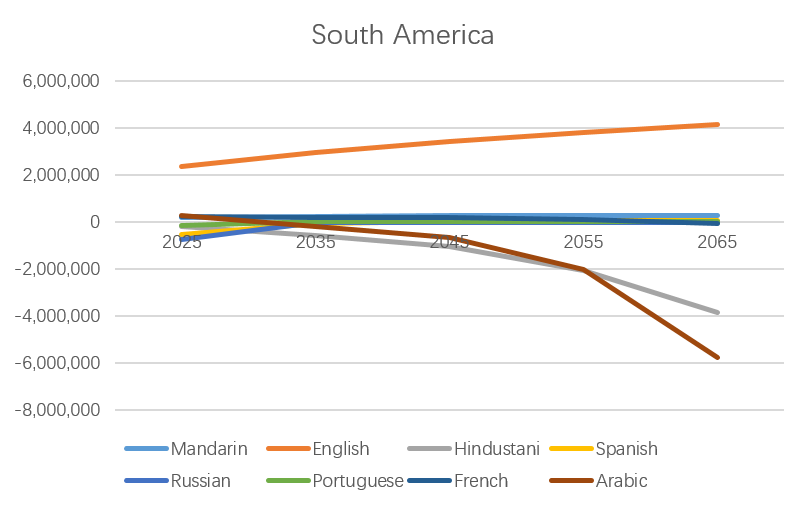
\includegraphics[height=3.8cm,width=6cm]{A05.png}%height=2.4cm,width=3.8cm
      \caption{\\Sorth America Language Distribution}
      \label{p12}
      \end{minipage}
      \begin{minipage}[t]{0.5\linewidth}
      \centering
      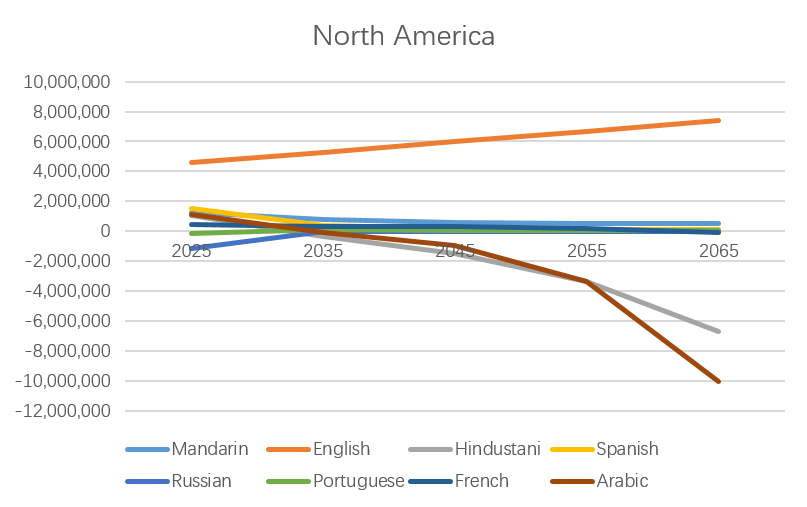
\includegraphics[height=3.8cm,width=6cm]{A06.png}%height=2.4cm,width=3.8cm
      \caption{\\North America Language Distribution}
      \label{p13}
      \end{minipage}
    \end{figure}

    As shown above, we can figure out that the trend of eight kinds of languages in Asia, Europe, North America, South America and Africa are basically the same.
    The distribution of English on these five continents will become more and more widespread, and its dissemination speed will also be faster.
    And there will be fewer people use Hindustani and Arabic in the five continents.
    As for Oceania, Hindustani will be used by more and more people in the future and fewer people will use Arabic.
    In all six continents, other languages have a tendency to distribute widespread, but at low speed.



    \subsection{Approximate Optimal Solution of 6 Offices}%6个办事处的近似最优解
    \subsubsection{Short Term}
    When considering short-term, we use 2016 data to calculate.

    We first seek the Standard Deviation of three different parameter distributions,
    and then use this as a weight to calculate the value of each region $w_i$.
    The results are shown in the following two tables:


    \begin{table}[h]
      \centering
      \caption{Standard Deviation at Present}

      \begin{tabular}{cc}
        \toprule%line
        &Standard Deviation\\
        \midrule%line
        Population&0.092167554\\
        GDP&0.094622429\\
        Language&0.79077675\\
        \bottomrule%line
      \end{tabular}
    \end{table}

    \begin{table}[h]
      \centering
      \caption{Value of Some Areas($w_i$)}

      \begin{tabular}{cc}
        \toprule%line
        Country or Area&Value($w_i$)\\
        \midrule%line
          China&0.060834\\
        America&0.053611\\
        India&0.79077675\\
        Arab League&0.037321031\\
        Brazil&0.009503611\\
        United Kingdom&0.009142346\\
        France&0.007572387\\
        Mexico&0.006997355\\
        Russian&0.006511811\\
        Canada&0.006258947\\
        \bottomrule%line
      \end{tabular}
    \end{table}

    Then given the initial solution, calculate the value of this program.
    And then the ninth country, Russia and 3-6 countries in turn exchange the value of the corresponding program.
    The corresponding data is as follows.
    \begin{table}[h]
      \centering
      \caption{Value of Iteration Before and After\ ($W$)}

      \begin{tabular}{ccccccc}
        \toprule%line
        Initial Solution&Change\ 1&Change\ 2&Change\ 3&Change\ 4&Change\ 5&Change\ 6\\
        \midrule%line
          12.1096&10.8703&11.9991&11.9086&11.2076&10.8399&10.2690\\
        \bottomrule%line
      \end{tabular}
    \end{table}

    The initial solution has the largest value, indicating that this scheme is a local optimal solution.
    Countries after the 9th place are less valuable and less likely to generate greater value than the initial solution.
    This program can be used as a program.
    Program as Figure 12 shown:

    \begin{figure}[h]
      \centering
      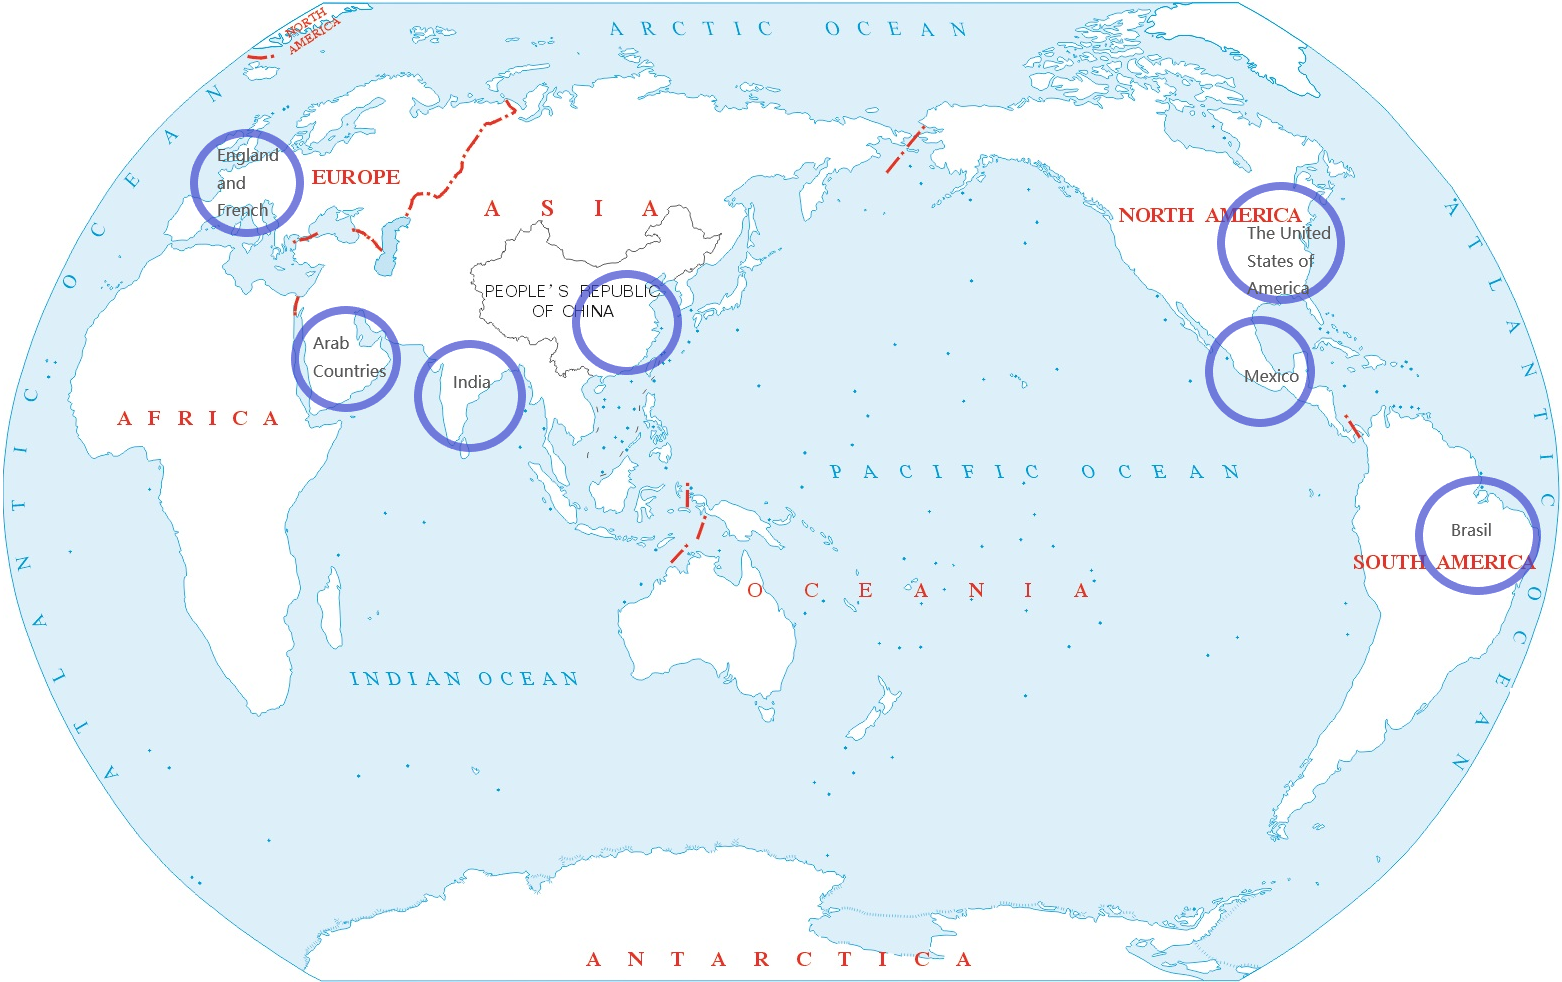
\includegraphics[height=6.3cm,width=10cm]{p8.png}
      \caption{Office selection location}
      \label{p14}
    \end{figure}

    \subsubsection{long Term}
    When considering long-term, we use the predicted data after 10 years and after 20 years.
    We use the same process as the short term.
    We calculate the Standard Deviatio and the regional value $W$.
    We use the same way to calculate two sets of values, the detailed data are as follows:

    \begin{table}[h]
      \centering
      \caption{Prediction after 10 Years: Value of Iteration Before and After\ ($W$)}

      \begin{tabular}{ccccccc}
        \toprule%line
        Initial Solution&Change\ 1&Change\ 2&Change\ 3&Change\ 4&Change\ 5&Change\ 6\\
        \midrule%line
          12.0673&10.8089&11.9461&11.9155&11.1252&11.2136&9.9886\\
        \bottomrule%line
      \end{tabular}
    \end{table}

    \begin{table}[h]
      \centering
      \caption{Prediction after 20 Years: Value of Iteration Before and After\ ($W$)}

      \begin{tabular}{ccccccc}
        \toprule%line
        Initial Solution&Change\ 1&Change\ 2&Change\ 3&Change\ 4&Change\ 5&Change\ 6\\
        \midrule%line
          11.7318&10.5858&11.6455&11.6141&10.7078&11.2164&9.7119\\
        \bottomrule%line
      \end{tabular}
    \end{table}

    Similarly, the initial solution can be used as the final solution.
    This program applies not only to short-term, but also to long-term.

    \subsection{Feasibility Study of Less Than 6 Offices}%少于6个办事处的可行性探究
    In designing the value function $W$, we have considered the impact of the number of offices on $W$.
    When setting up five offices, the formula for $W$ becomes as follows:
    $$W=\sum_{i=1}^7(w_i\frac{\sum_{j=1,j\neq i}^7 d_{ij}}{7})$$

    We do the conversion based on the above feasible solution.
    We have six separate offices removed. Calculate the value of W after removing an office.
    The calculation results are as follows:

    \begin{table}[h]
      \centering
      \caption{Value of Remove Before and After\ ($W$)}

      \begin{tabular}{ccccccc}
        \toprule%line
        Original Solution&Remove\ 8&Remove\ 7&Remove\ 6&Remove\ 5&Remove\ 4&Remove\ 3\\
        \midrule%line
          12.1096&11.0628&12.2628&12.1643&11.4451&10.9979&10.3993\\
        \bottomrule%line
      \end{tabular}
    \end{table}

    When 7 is removed, W gets the maximum.
    This shows that we can remove the No. 7 country office. We can cancel the office in Mexico.
    In this model, fewer than six offices are possible.

  \section{Sensitivity Analysis---A Case Study in English}
  As we said before, we use a fixed diffusion coefficient $D$ and a fixed number of iterations to predict the situation 50 years later.
  Then we discuss what impact these two factors will have on the outcome of the forecast.

    \subsection{GDP Changes Lead to $D$ Changes}
    As we said before,
    we consider the impact of Immigration, GDP and Language Family on the Diffusion Coefficient D.
    It is determined by the following formula:
    $$D=\beta_1\times Imm+\beta_2\times GDP+\beta_3\times LF$$

    We try to introduce changes in GDP to cause changes in $D$.
    The number of iterations is still 5 times.
    The diffusion coefficient $D$ of each iteration will change with the change of GDP in the corresponding period of time.
    We give GDP data a 10-year growth rate.
    We change this growth rate to observe the changes in the forecast results.
    The following is the result of our given growth rates of 3\%, 6\% and 9\% per 10 years respectively.

    \begin{figure}[h]
      \centering
      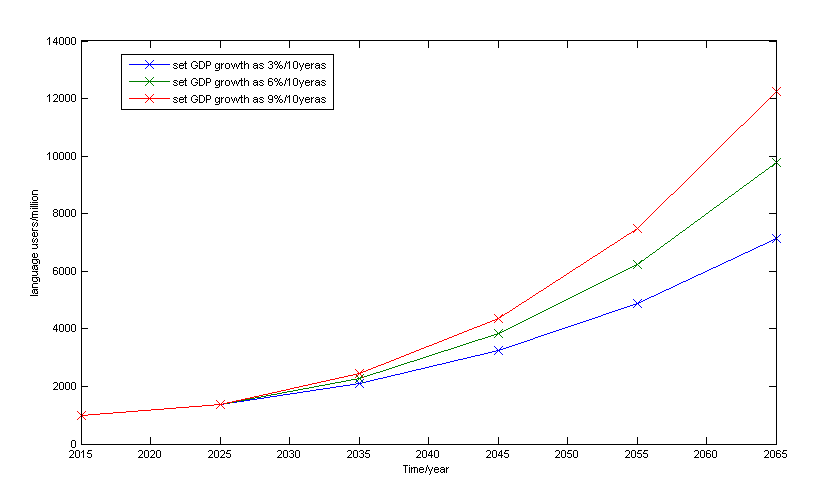
\includegraphics[height=6.3cm,width=10cm]{p6.png}
      \caption{GDP Changes Lead to Prediction Changes}
      \label{p6}
    \end{figure}
      %\subsubsection{Population}

      %\subsubsection{GDP}

      %\subsubsection{Immigration}

    %\subsection{Quantification of Diffusion Coefficient $D$}

    \subsection{Influence of Iteration Number }%迭代结果
    We explore the impact of the number of iterations on the prediction.
    Without changing other parameters, only change the number of iterations.
    The figure below shows the forecast after 50 years with iterations of 1, 2, 5 and 10.

    \begin{figure}[h]
      \centering
      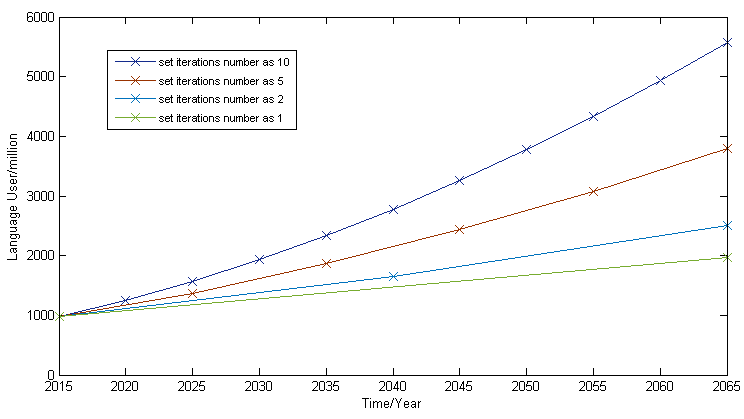
\includegraphics[height=6.3cm,width=10cm]{p5.png}
      \caption{Influence of Iteration Number}
      \label{p5}
    \end{figure}

    The greater the number of iterations, the greater the prediction.
    Too small a number of iterations will make the prediction far below the actual value.
    When applying the model to calculate the actual situation should choose the appropriate number of iterations.


  %\section{Sensitivity Analysis}

    %\subsection{Influence of the Upper Limit Parameter $k$}
    %When $k$ takes different values,
    %we find that the effects of diffusion coefficients $D_1$ and $D_2$
    %for the two time periods of 2013 ~ 2015 and 2015 ~ 2017 are as follows:

    %We can easily see that the value of k does not affect the ratio between the two diffusion coefficients.
    %$k$ does not affect the proportionality of $D$.
    %We only need to find a suitable k so that the value of D is in the right range.


    %\subsection{Number of Iterations}

  \section{Conclusions}
  According to our model, the change of population, similarities between different languages, immigration and economic conditions all play important role in language transmission.
  The similarities between different languages are related to language family.
  If both the mother tongue and the second language belong to the same language family, learning a second language is much easier.
  The economy is the basis for the other elements.
  The more developed the economy, the more immigrants moved in.
  Economic development also affects government policies and business exchanges.
  The economy is closely linked with the spread of language.

  And we find that the number of English speaker grow faster than any other language in the next fifty years.
  Arabic and Hindustani will also develop rapidly in future,
  while other languages will not have much change.
  In particular, although China is making great efforts to promote Chinese,
  learning Chinese is extremely difficult.
  In addition, people predict that the population of China will show a contracted state in the future, and the number of native speakers will decrease.
  These lead to the rapid development of Chinese will not.

  In different continents, the language distribution changes are not the same.
  The development of English in each big state is very fast.
  Hindi and Arabic generally show the downturn trend.
  And the development of other languages is very flat.

  Based on the results of our iteration,
  the best programs in 20 years will remain unchanged
  if we set up six additional international offices.
  We recommend that multinational service companies
  set up offices in the United Kingdom, India, the Arab region, France, Mexico and Brazil.
  When only five offices could be set up,
  the program to remove the Mexico office would be more effective than the original six office programs.
  If we only consider the location's
  value to the company and the distance among the offices, according to our results, it's feasible to set less than six offices.

  \section{Strengths and Weaknesses}
  \subsection{Strengths}
  \begin{itemize}
    \item\textbf{Easy to promote:} \\
    The included parameters of our model have a greater impact on the predicted results. In the case of immigration,
    GDP and population changes, the forecast value will also change, reflecting the objective laws.
    Also, choosing an iterative method to solve the problem of location can avoid the heavy workload when using the enumeration method.
    \item\textbf{Diffusion model concise and intuitive:} \\
    Diffusion model Analog ink drip into water, easy to understand.
    Since the final formula is very simple,
    the calculation of the model does not require too much computation and complicated calculation methods.
  \end{itemize}
  \subsection{Weaknesses}
  \begin{itemize}
    \item\textbf{Many predictors:} \\
    The model's predictions are based on a few predictors.
    The forecast of these forecasts is not enough objective and accurate.
    The forecast result has big deviations compared with the real value.
    \item\textbf{Iteration site is not comprehensive:}\\
    Iterative method does not traverse each possibility.
    We are likely to miss the global optimal solution.
  \end{itemize}

  \section*{References}
  \addcontentsline{toc}{section}{References}
  \begin{enumerate}
  \item Xiaolan, Song, Xuehui, Huang. Fundamentals of Inorganic Materials Science[M]. Beijing:Chemical Industry Press, 2005.
  \item Gengxiang, Hu, Xun, Cai. Fundamentals of Materials Science[M]. Shanghai:Shanghai Jiao Tong University Press, 2009.
  \item DEPARTMENT OF STATE\ \ Foreign Language Proficiency Has Improved, but Efforts to Reduce Gaps Need Evaluation \\
  \url{https://www.gao.gov/assets/690/683533.pdf}\\
  \item United Nations\ \ World Population Prospects The 2015 Revision \\
  \url{https://esa.un.org/unpd/wpp/Publications/Files/Key_Findings_WPP_2015.pdf}\\
  \item International Organization for Migration\ \ WORLD MIGRATION REPORT 2018 \\
  \url{https://publications.iom.int/system/files/pdf/wmr_2018_en.pdf}\\
  \end{enumerate}

  \section*{Memo}
  \addcontentsline{toc}{section}{Memo}
  \ \\
  To:Chief Operating Officer\\
  From: Modeling team 85691\\
  Date: 12 February 2018\\
  Subject: Location options for new offices\\

  We'd like to remind you that,according to our analysis,
  In the next 50 years, there is a distinct advantage in the growth of English speakers over other languages.
  A few languages have a faster rate of diffusion,
  others are slower and similar.
  Considering economy,
  population and the attribute of language, among the results of our analysis, China, the United States, India and the Arab League countries
  are most suitable for setting up new offices,
  which can bring more benefits to the company than other countries.
  However, considering the rational allocation of resources,
  If you want to set up six offices,
  we will recommend the United Kingdom, India, the Arab region, France, Mexico, Brazil as a candidate.
  To reduce the number of offices set up,
  Mexico first became an option.
  Compared with the other five countries,
  the removal of Mexico has the least effect on the overall benefit and can even be neglected.
  Based on this, there is no need to set up too much office.
  Apparently, as time goes on, the number of people who use English has greatly increased, technology continues to progress,
  the impact of language barrier on the office's choice of address will be getting smaller and smaller.
  Therefore, the benefits of setting up a new office are more of a benefit in the short term,
  and you should think in this light.














\end{document}
